\chapter{Research Goals}
\label{cha:ResearchGoals}

The goal of this thesis is to contribute in the domain of autonomous driving by investigating the use of reinforcement learning to train an autonomous driving agent that is resilient to changes in light conditions. The agent is evaluated on  simulated parcours that consist of a series of goals indicated by two blocks, a parcour is successfully completed if the agents drives through all goals without collisions.
This thesis builds upon previous work at the ScaDS.AI \textcite{maximilian} and uses the same parcour and task specifications. The agent from previous work was not able to reliably complete parcours under changing light conditions, motivating the research goals of this thesis.


The self-driving agent is trained using reinforcement learning in a simulated environment, the training process will include changing light conditions and possibly data augmentation to help the agent generalize.
Parcours of different difficulties and lighting settings are used to evaluate the agent's reliability and generalisation capabilities. The most important evaluation metric is the success rate. A parcour is considered a success when the autonomous driving agent passes all goals without any collisions.


\begin{figure}
    \centering
    \subfigure{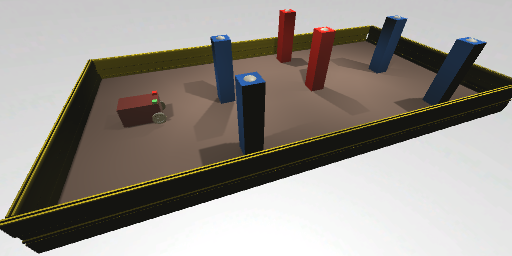
\includegraphics[width=0.4\textwidth]{Bilder/image_printer_images/evaluation_hard.png}}\qquad
    \subfigure{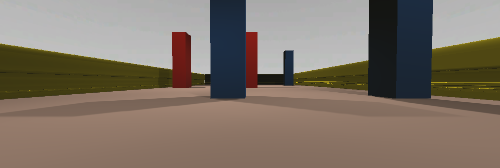
\includegraphics[width=0.4\textwidth]{Bilder/image_printer_images/agent_image_from_unity.png}}\\
    \caption{Example image of a parcour and the agent's camera}
\end{figure}


\section{Question 1 - \questionOne}

The previous work \textcite{maximilian} showed that it is possible to train an agent using reinforcement learning to solve the evaluation parcours, however the trained agents were not successful in reliably traversing the parcours of higher difficulty levels. Furthermore this work will implement the agent in a fundamentally different way, the agents developed in previous work utilized an extensive preprocessing pipeline to extract the relevant information from the camera images whereas the agents in this thesis will use a convolutional neural network to learn and extract the relevant information themselves.

Due to these differences in implementation and as a prerequisite for question 2 and 3, it is first important to investigate if it is possible to train an agent to reliably solve the parcours of all difficulty levels. This raises question 1:
\questionOne

The question will be answered by training agents that have been developed based on related work and analyzing their performance on the evaluation parcours. The evaluation parcours consist of different difficulty levels, the agent's success rate will be primarily used to answer the question.


\section{Question 2 - Is it possible to use an end-to-end trained CNN to make the agent robust to changing light conditions?}

While question 1 simply investigates if it is possible to train an agent to reliably solve the parcours of all difficulty levels, question 2 investigates if it is possible to train an agent that is robust to changing light conditions in addition to being capable of solving parcours of all difficulty levels. The performance of agents from previous work \textcite{maximilian} declined massively under changing light conditions. This raises question 2 - \questionTwo

The question will be answered by training agents that have been specifically designed to be robust to changing light conditions, the agents will be trained using reinforcement learning in a simulated environment with changing light conditions and possibly further data augmentation to help the agent generalize and learn. The agents will be evaluated on the evaluation parcours used in question 1 with changing light conditions. Similarly the success rate will be primarily used to evaluate and compare the agent's performance. The difference in performance for different light conditions will be used to answer the question, if the performance is similar for all light conditions the agent is considered robust to changing light conditions.

\section{Question 3 - \questionThree}

One goal of the ongoing research at the ScaDS.AI is to build real life robots for demonstration and research purposes \textcite{merlin_flach}, the robots are based on the NVIDIA JetBot platform. The robots are equiped with a camera, wheels and a small computer. A future goal is to transfer a trained agent onto these robots, however the limited processing power of these robots might not be sufficient for more complex agents that utilize neural networks. This raises question 3 - \questionThree


The question will be answered by investigating the processing power required to run the preprocessing steps and neural networks used in the agents that are developed in this thesis. This will be evaluated empirically by creating replays of the agents in simulations and running these replays on the physical robots. If the robots are able to reproduce the behaviour from the replays, the agents can be considered transferable to the robots.

TODO read this chapter xD
TODO abgrenzung und motivierung hervorheben